\documentclass[12pt]{article}

\usepackage{graphicx}

\usepackage[round]{natbib}
\usepackage{hyperref}
\usepackage{color}
\usepackage{gb4e}
\usepackage{subcaption}
\usepackage{multicol}

\usepackage{stmaryrd}

\newcommand{\mvalueof}[1]{\llbracket#1\rrbracket}

%%%New commands%%%
\newcommand{\tuple}[1]{\ensuremath{\left\langle #1 \right\rangle}} 
\newcommand{\citeposs}[2][]{\citeauthor{#2}'s (\citeyear[#1]{#2})}
\newcommand{\hloranj}[1]{\textcolor[rgb]{.8,.33,.0}{#1}}% prints in orange
\newcommand{\hlblue}[1]{\textcolor[rgb]{0.13,0.67,0.8}{#1}}
\newcommand{\hlgrey}[1]{\textcolor[rgb]{0.57, 0.64, 0.69}{#1}}

%\DeclareMathOperator*{\argmax}{arg\,max}
\newcommand{\argmax}[1]{\underset{#1}{\operatorname{arg}\,\operatorname{max}}\;}
\newcommand{\argmin}[1]{\underset{#1}{\operatorname{arg}\,\operatorname{min}}\;}

\newcommand*{\defeq}{\mathrel{\vcenter{\baselineskip0.5ex \lineskiplimit0pt
                     \hbox{\scriptsize.}\hbox{\scriptsize.}}}%
                     =}

	%%%%%%%%%%%%%%%%%%
\usepackage{mathcomp}
\usepackage{blkarray} %to label matrix
\usepackage{amssymb}
\usepackage{amsmath}
\usepackage{hyperref}
\usepackage{nicefrac}

\begin{document}


\title{Comparison between iterated learning and fitness+learning}
\date{\today}

\maketitle

For comparability, we follow the setup analyzed by \citet[\S 6]{griffiths+kalish:2007} on the emergence of compositionality. $S = \{00,01,10,11\} = M$. $\mathcal{L}$ is the set of all possible mappings from $S$ to $M$, i.e. $4^4 = 256$ possible signaling systems.\footnote{Note that \citet{griffiths+kalish:2007} only take one-to-one mappings into consideration.} Four of which are compositional in that meaning and form components agree position-wise.\footnote{Note that \citet{griffiths+kalish:2007} take $260$ languages into consideration. $256$ possible (holistic) languages and $4$ compositional ones. However, the former set includes $4$ `holistic' languages identical to the $4$ compositional ones. In contrast, we consider $252$ holistic and $4$ compositional languages. (N.B.: They include 4 languages holistic languages indistinguishable from their compositional counterparts to show that the learning bias drives selection. We already know that, so it's not necessary.)} Syntax, i.e. component order, is assumed to be given. $P(s) = \nicefrac{1}{|S|}$. The simulations involve a (hierarchical) prior parameter $\alpha \in [.01,0.5]$, an error parameter $\epsilon \in [.01,.05]$ and data length $n \in [1,10]$.
\vspace{1cm}

Hierarchical prior:
\begin{align}
P(L) &= \left\{\begin{array}{l} \frac{\alpha}{4} \qquad \textnormal{if $L$ is compositional}\\
\frac{1 - \alpha}{252} \quad \textnormal{otherwise}\end{array}\right.
%U_S(t_i, m_j, a_k) &= U_R(t_i, m_j, a_k)
\end{align}

Production: 
\begin{align}
P(m|s,L) &= \left\{\begin{array}{l} 1 - \epsilon \qquad \textnormal{if $m$ is true of $s$ in $L$}\\
\frac{\epsilon}{3} \quad \  \qquad \textnormal{otherwise}\end{array}\right.
%U_S(t_i, m_j, a_k) &= U_R(t_i, m_j, a_k)
\end{align}


Interpretation (not covered by \citealt{griffiths+kalish:2007}):
\begin{align}
P(s|m,L) \propto P(s) P(m|s,L)
\end{align}

\paragraph{Results.} The following plots exemplify the main differences between iterated learning and evolutionary game theory with Bayesian learning. Each dynamic was run with learning as sampling from the posterior ({\em post-sampling}) as well as with learning as maximum posterior likelihood ({\em MAP}). Furthermore, we include results for both parental learning (standard mutation) and communal learning (weighted mutation) for the EGT variant. All quantities were subjected to a square root transformation to make the differences between these variants more apparent-- in particular for the quantities of holistic languages that remain under each variant. The parameter values correspond to those reported by \citealt[466]{griffiths+kalish:2007} (rightmost plots), therefore, the results from iterated learning with posterior sampling as well as the prior double as a replication of their setup.

To ensure comparability, we also follow Griffiths \& Kalish in running all simulations for $10000$ generations and taking an average of $1000$ such games for each parameter value and variant of dynamics/learning.

\paragraph{Simulation 1.} $\alpha = 0.5, \epsilon = 0.05, n = 1$. Observations: 


\begin{figure}[h!]
\makebox[\linewidth][c]{%
\begin{subfigure}[b]{.7\textwidth}
\centering
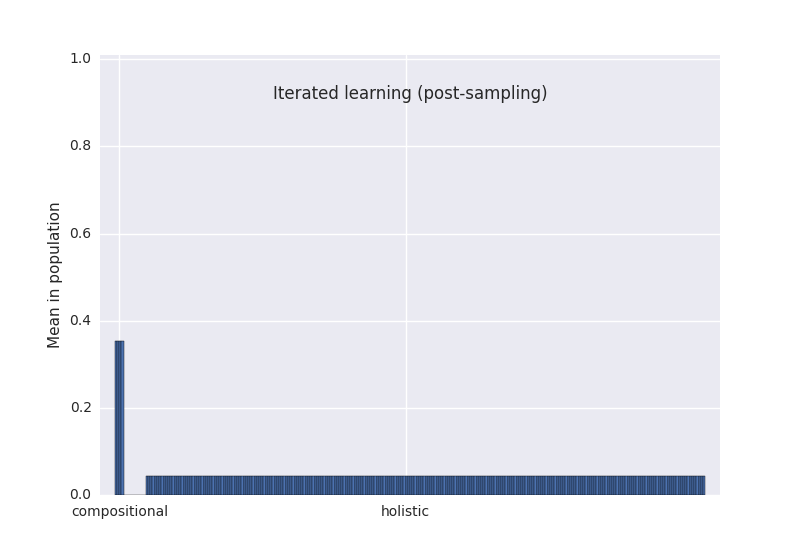
\includegraphics[scale=0.5]{./plots/test1}
%\caption{a test subfigure}
\end{subfigure}%
\begin{subfigure}[b]{.7\textwidth}
\centering
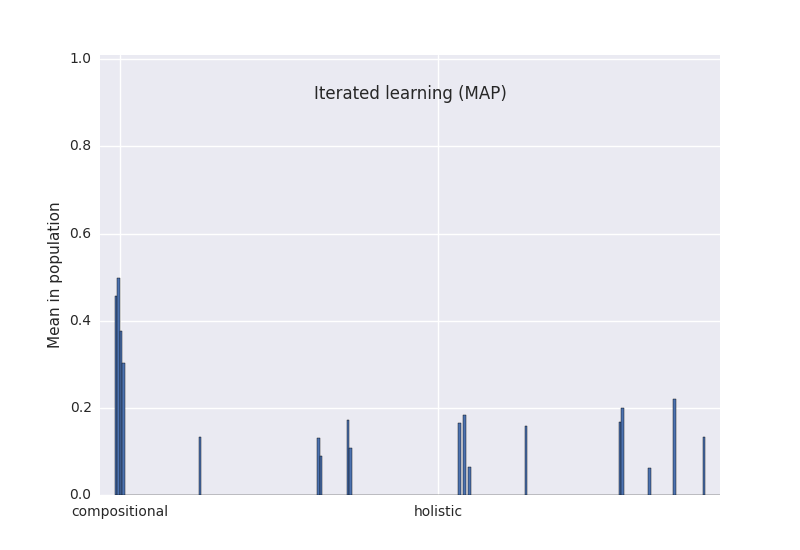
\includegraphics[scale=0.5]{./plots/test2}
%\caption{a test subfigure}
\end{subfigure}%
}
\end{figure}

\paragraph{Simulation 2.} $\alpha = 0.5, \epsilon = 0.05, n = 1$
\paragraph{Simulation 3.} $\alpha = 0.5, \epsilon = 0.05, n = 1$
\paragraph{Simulation 4.} $\alpha = 0.5, \epsilon = 0.05, n = 1$


\bibliographystyle{unsrtnat}

\bibliography{../../Dropbox/tex/masternolinks}



\end{document}
